\subsubsection{29.11.14}

\begin{enumerate}
	\item The time of beginning and ending of the meeting:
	16:00 - 20:10
	\item Purposes of the meeting:
	\begin{enumerate}
		\item To finish the alteration of MEL.
		
		\item To elaborate concept of the new gripper for balls.
		
		\item To test the MEL.
		
	\end{enumerate}
	\item Work, that has been done:
	\begin{enumerate}
		\item MEL was finished. Now it moves by four motors with gear ratio 1:1.
		
		\begin{figure}[H]
			\begin{minipage}[h]{0.2\linewidth}
				\center  
			\end{minipage}
			\begin{minipage}[h]{0.6\linewidth}
				\center{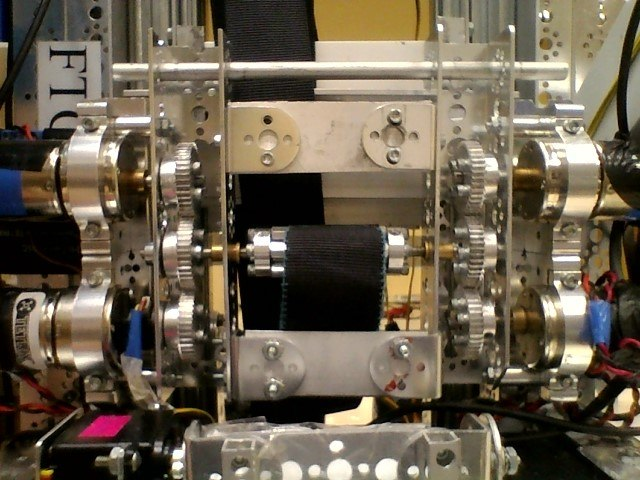
\includegraphics[scale=0.3]{days/29.11.14/images/01}}
				\caption{Changed MEL}
			\end{minipage}
		\end{figure}
		
		\item MEL was tested. Speed of extracting increased twice. Motors not experiences undue stress during the working.
		
		\item Ties has too small stiffness and not always captures balls and often break. It was decided use blades that cut from the plastic bottle. It was designed that optimal count of blades - 3. In addition it was decided to improve the bucket so that the bucket has a ramp 7cm in hight in the front part. It will allow to us capture 5 big balls. Also the balls will not fall from the bucket. It was created schematic drawing of gripper and bucket.
		
		\begin{figure}[H]
			\begin{minipage}[h]{0.2\linewidth}
				\center  
			\end{minipage}
			\begin{minipage}[h]{0.6\linewidth}
				\center{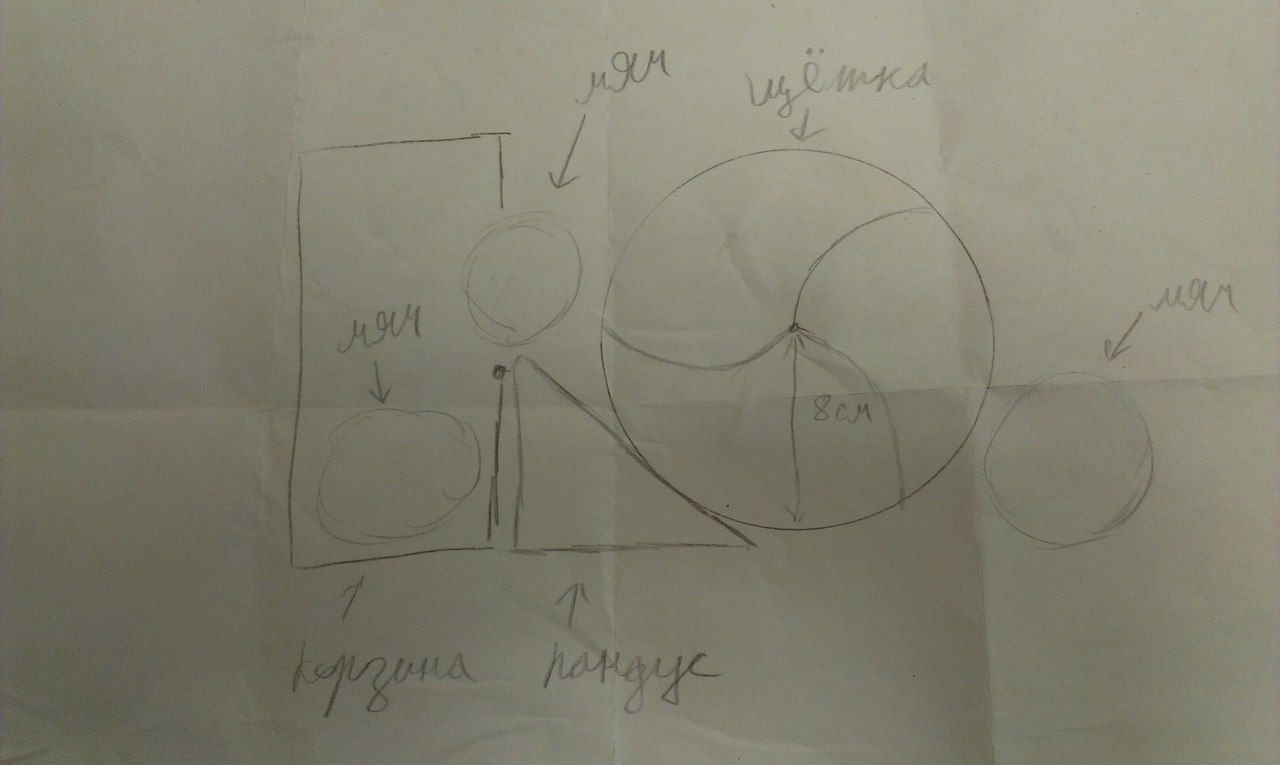
\includegraphics[scale=0.2]{days/29.11.14/images/02}}
				\caption{Drawing of gripper and bucket}
			\end{minipage}
		\end{figure}
		
	\end{enumerate}
	
	\item Results:
	\begin{enumerate}
		\item The alteration of MEL was finished.
		
		\item MEL was tested. The speed of rising increased twice.
		
		\item Construction of new gripper for balls was elaborated.
		
	\end{enumerate}
	
	\item Tasks for the next meetings:
	\begin{enumerate}
		\item To change the gripper for balls.
		
	\end{enumerate}     
\end{enumerate}
\fillpage